\documentclass[12pt]{article}

% Setting up the page
\usepackage{setspace}
    \newcommand{\standardspacing}{\singlespacing}
    \standardspacing%
\usepackage[english]{babel}
\usepackage[utf8]{inputenc}
\usepackage{fullpage}

% Bibliography
\usepackage[numbers]{natbib}
\bibliographystyle{plain}

% Writing mathematics, algorithms and code
\usepackage{mathtools}
\usepackage{amsmath}
\usepackage{amssymb}
\usepackage[boxruled]{algorithm2e}

\newcommand{\balg}[1][htbp]{%
    \begin{algorithm}[#1]\DontPrintSemicolon\singlespacing%
}
\newcommand{\ealg}{%
    \end{algorithm}\standardspacing%
}

\newcommand{\true}{\text{True}}
\newcommand{\false}{\text{False}}
\DeclareMathOperator*{\argmax}{arg\,max}
\DeclareMathOperator*{\argmin}{arg\,min}

\DeclarePairedDelimiter\abs{\lvert}{\rvert}%
\DeclarePairedDelimiter\norm{\lVert}{\rVert}%

% Importing images, tables and referencing
\usepackage{graphicx}
\usepackage{tikz}
\usepackage{xcolor}
\usepackage[colorlinks=true,
            linkcolor=black,
            urlcolor=blue,
            citecolor=black,
            anchorcolor=black]{hyperref}
\usepackage{caption}
\usepackage{booktabs}
\usepackage{float}

% For indexing sections, etc.
\usepackage{amsthm}
\theoremstyle{definition} \newtheorem{definition}{Definition}[section]
\newtheorem*{remark}{Remark}
\newtheorem{theorem}{Theorem}

\newtheoremstyle{example}
{\topsep} % Space above
{\topsep} % Space below
{} % Body font (normal)
{} % Indent
{\bfseries} % Head font
{.} % Punctuation after head
{.5em} % Space after head
{} % Head spec (normal)

\theoremstyle{example} \newtheorem{example}{Example}

\title{%
    A novel game-theoretic initialisation process for the \(k\)-modes
    algorithm using the hospital-resident assignment problem
}
\author{Henry Wilde, Vincent Knight and Jonathan Gillard}

\begin{document}

\maketitle%
\begin{abstract}
    This paper presents a new way of selecting an initial solution for the
    \(k\)-modes algorithm that allows for a notion of game theoretic fairness
    that classic initialisations, namely those by Huang and Cao, do not. The
    method, which utilises the Hospital-Resident Assignment Problem to find the
    set of initial cluster centroids, is compared with two initialisation
    methods for \(k\)-modes~\cite{Huang1998} as well as the next most popular
    method present in the literature~\cite{Cao2009}. In order to highlight the
    merits of the proposed method two stages of analysis are presented. The
    paper concludes with an analysis of these methods against the proposed and
    it is demonstrated that the proposed method is able to outperform them both.
    The aim of this analysis is two-fold: first, to highlight the merits of the
    method in a familiar setting by clustering well-known benchmark datasets;
    and second, to provide a deeper insight into how the methods perform against
    one another by generating artificial datasets using the method set out
    in~\cite{Wilde2019}.
\end{abstract}

\clearpage%

\abstract{
The \(k\)-modes algorithm is a part of the family of clustering algorithms known
as `prototype-based clustering', and is an extension of the \(k\)-means 
algorithm for categorical data as set out in~\cite{Huang98}. This work will 
outline the key differences and similarities between two established
initialisation methods for the \(k\)-modes algorithm, and in doing so we will be
able to examine how the initial cluster selection process has an impact on the 
efficiency and quality of the \(k\)-modes algorithm. From there, we will define
a new initialisation method that makes use of elements of game theory.
}

\clearpage

\section{The \(k\)-modes algorithm}\label{sec:kmodes}

\subsection{Notation}\label{subsec:notation}

We will use the following notation throughout this work to describe our dataset,
its points, our clusters and their representative points:

\begin{itemize}
    \item Our dataset has \(N\) elements and is denoted by \textbf{X}.
    \item \textbf{X} is described by a set of \(m \in \mathbb{Z}_+\) attributes 
        \(\textbf{A} = \{A_1, \ldots, A_m\}\).
    \item Each attribute \(A_j\) is considered as a set of attribute values 
        \(A_j = \{a_1^{(j)}, \ldots, a_{d_j}^{(j)}\}\) where \(d_j = |A_j| \in 
        \mathbb{Z}_+\) is sometimes used as shorthand for the size of the 
        \(j^{th}\) attribute set.
    \item We write each data point \(X^{(i)}, \ i = 1, \ldots, N\), as an 
        \(m\)-dimensional vector:
	    \[
		    X^{(i)} = \left[x_1^{(i)}, x_2^{(i)}, \ldots, x_m^{(i)}\right], \
            \text{where} \ x_j^{(i)} \in A_j \ \text{for all} \ j = 1, \ldots, 
            m.
	    \]
        Here, we refer to \(x_j^{(i)}\) as the value of the \(j^{th}\) attribute
        of the \(i^{th}\) data point, \(X^{(i)}\). A tabular representation is 
        given below:
        \begin{table}[H]
        \centering
        \begin{tabular}{cccccc}
            {} & \(A_1\) & \(A_2\) & \quad \ldots \quad & \(A_{m-1}\) & \(A_m\)
            \\
            \midrule
            \(X^{(1)}\) & \(x_1^{(1)}\) & \(x_2^{(1)}\) & \quad \ldots \quad & 
            \(x_{m-1}^{(1)}\) & \(x_m^{(1)}\)
            \\
            \(X^{(2)}\) & \(x_1^{(2)}\) & \(x_2^{(2)}\) & \quad \ldots \quad &
            \(x_{m-1}^{(2)}\) & \(x_m^{(2)}\)
            \\
            \vdots & \vdots & \vdots & {} & \vdots & \vdots
            \\
            \(X^{(N)}\) & \(x_1^{(N)}\) & \(x_2^{(N)}\) & \quad \ldots \quad &
            \(x_{m-1}^{(N)}\) & \(x_m^{(N)}\)
            \\
        \end{tabular}
        \end{table}
	\item Prototype-based clustering algorithms partition the elements of 
        \(\textbf{X}\) into \(k\) distinct sets (which we call clusters) denoted
        by \(C_1, \ldots, C_k\), where \(k \in \mathbb{Z}_+\) is a 
        pre-determined, fixed integer such that \(k \le N\). That is:
	    \[
		    C_1, \ldots, C_k \ \text{are such that} \ \bigcup_{l=1}^k C_l = 
		    \textbf{X} \quad \text{and} \quad C_l \cap C_t = \emptyset \
		    \text{for all} \ l \neq t
	    \]
    \item Each cluster \(C_l\) has associated with it a representative point 
		(see Section~\ref{subsec:rep-points}) which we denote by 
        \(\mu^{(l)}~=~\left[\mu_1^{(l)},~\ldots,~\mu_m^{(l)}\right]\). These
        points are also referred to as cluster centers, modes and centroids.
\end{itemize}


\subsection{Dissimilarity measure}\label{subsec:dissim}

An immediate difference between the \(k\)-means and \(k\)-modes algorithms is 
that they deal with different types of data, and so the metric used to define 
the distance between two points in our space must be different. With 
\(k\)-means, where the data has all-numeric attributes, Euclidean distance is 
often used. However, we do not have this sense of distance with categorical 
data. Instead, we utilise a dissimilarity measure \-- defined below \-- as our 
metric. It can be easily checked that this is indeed a distance measure.

\begin{definition}\label{def:dissim}
    Let \(\textbf{X}\) be a dataset and consider \(X^{(a)}, X^{(b)} \in
    \textbf{X}\). We define the \emph{dissimilarity} between \(X^{(a)}\) and 
    \(X^{(b)}\), denoted by \(d(X^{(a)}, X^{(b)})\), to be:
    \[
        d(X^{(a)}, X^{(b)}) = \sum_{j=1}^{m} \delta(x_j^{(a)}, x_j^{(b)}) \quad
        \text{where} \quad \delta(x, y) = \begin{cases}
                                              0, & \text{if} \ x = y \\
			    		                      1, & \text{otherwise}
				    	                  \end{cases}
    \]

    In other words, the dissimilarity between two points is simply the number of
    attributes where their values are not the same. It should also be clear that
    the dissimilarity between a point and itself is always zero.
\end{definition}


\begin{example}\label{ex:dissim}
    Throughout this work, we will make use of a number of small examples to aid
    our understanding of various concepts. These examples will utilise a small,
    artificial dataset describing some qualities about vehicles.
    
    The dataset is made up of \(N = 10\) instances, each of which describe a
    vehicle. These instances are defined by \(m = 6\) attributes, the first two
    of which are ordinal variables taken from the set \(\{\text{L, M, H, V}\}\)
    standing for `low', `medium', `high', and `very high', respectively. The
    next three are integer variables and so can be considered as categorical,
    and the final attribute is a binary variable indicating whether the vehicle
    is eco-friendly \((1)\) or not \((0)\). The full dataset is given in
    Table~\ref{tab:dataset}. Please note that there is an additional, unheaded
    column on the left hand side showing the index starting at \(1\) and going
    up to \(5\).
    
    \begin{table}[H]
        \centering
        \singlespacing{%
        \resizebox{.8\textwidth}{!}{%
            \centering
            \begin{tabular}{lllrrrr}
\toprule
{} & Price & Maintenance &  Doors &  Passengers &  Wheels &  Eco-Friendly \\
\midrule
0 &     H &           M &      2 &           2 &       4 &             0 \\
1 &     L &           M &      0 &           1 &       2 &             0 \\
2 &     V &           H &      2 &           3 &       8 &             0 \\
3 &     H &           L &      4 &           5 &       4 &             1 \\
4 &     M &           M &      2 &           5 &       4 &             1 \\
5 &     M &           L &      2 &           4 &       4 &             1 \\
6 &     V &           H &      4 &           5 &       4 &             0 \\
7 &     L &           V &      2 &           4 &       4 &             0 \\
8 &     H &           M &      0 &           2 &       2 &             1 \\
9 &     H &           M &      4 &           7 &       4 &             0 \\
\bottomrule
\end{tabular}

        }}
        \caption{The vehicle dataset.}\label{tab:dataset}
    \end{table}

    Let us consider our first two datapoints. With the notation laid out in
    Section~\ref{subsec:notation}, we can express these points as vectors in the
    following way:

    \begin{equation}
        \nonumber
        \begin{aligned}
            X^{(1)} & = & \left[ x_1^{(1)} = \text{H}, \ x_2^{(1)} = \text{M}, \
            x_3^{(1)} = 2, \ x_4^{(1)} = 2, \ x_5^{(1)} = 4, \ x_6^{(1)} = 0 
            \right]
            \\
            X^{(2)} & = & \left[ x_1^{(2)} = \text{L}, \ x_2^{(2)} = \text{M}, \
            x_3^{(2)} = 0, \ x_4^{(2)} = 1, \ x_5^{(2)} = 2, \ x_6^{(2)} = 0
            \right]
        \end{aligned}
    \end{equation}

    Then, by Definition~\ref{def:dissim}, their pairwise dissimilarity is:
    \begin{equation}
        \nonumber
        \begin{aligned}
            \centering
            d(X^{(1)}, X^{(2)}) & = & \delta(\text{H}, \text{L}) & + & 
            \delta(\text{M}, \text{M}) & + & \delta(3, 0) & + & \delta(2, 1) &
            + & \delta(4, 2) & + & \delta(0, 0) & {} & {}
            \\
            {} & = & 1 \ & + & 0 \ & + & 1 \ & + & 1 \ & + & 1 \ & + & 0 \ & = &
            4
        \end{aligned}
    \end{equation}
\end{example}

\subsection{Representative points}\label{subsec:rep-points}

Now that we have defined a metric on our space, we can turn our attention to
what we mean by the representative point \(\mu^{(l)}\) of a cluster \(C_l\). In
\(k\)-means, these representative points are called centroids or cluster centers
and are defined to be the average of all points \(X^{(i)} \in C_l\). With
categorical data, we use our revised distance measure from
Definition~\ref{def:dissim} to specify a representative point. We typically call
these points a mode of \textbf{X}.

\begin{definition}\label{def:mode}
    We define a \emph{mode} of our set \textbf{X} to be any vector \(\mu =
    [\mu_1, \ldots, \mu_m]\) that minimises the \emph{summed dissimilarity}:

    \begin{equation}
        D(\textbf{X}, \mu) = \sum_{i=1}^{N} d\left(X^{(i)}, \mu\right)
    \end{equation}
	
    Note that \(\mu\) is not necessarily in \textbf{X}, and in this case we call
    \(\mu\) a \emph{virtual mode} of \textbf{X}.
\end{definition}

\begin{definition}\label{def:rel-freq}
    Let \textbf{X} be a dataset with attributes \(A_1, \ldots, A_m\). Then we
    denote by \(n(a_s^{(j)})\) the \emph{frequency} of the \(s^{th}\) category
    \(a_s^{(j)}\) of \(A_j\) in \textbf{X}. That is:

    \[
        n(a_s^{(j)}) := \abs*{{\{X^{(i)} \in \textbf{X}: x_j^{(i)} =
        a_s^{(j)}\}}}
    \]
	
    We call \(\frac{n(a_s^{(j)})}{N}\) the \emph{relative frequency} of category 
    \(a_s^{(j)}\) in \textbf{X}.
\end{definition}

\begin{remark}
    Note that we have \(1 \le n(a_s^{(j)}) \le N\) for all \(s\) and
    \(j~=~1,~\ldots,~m\).\\
\end{remark}

\begin{theorem}\label{thm:1}
    Consider a dataset \textbf{X} and some \(X^{(i)} \in \textbf{X}\). Then:
    \[
	    D(\textbf{X}, X^{(i)}) \ \text{is minimised} \ \iff n(x_j^{(i)}) \geq 
	    n(a_s^{(j)}) \ \text{for all} \ s~=~1,~\ldots,~d_j \ \text{for each} \
        j~=~1,~\ldots,~m.
    \]
    A proof of this theorem can be found in the Appendix of~\cite{Huang98}.
\end{theorem}

\begin{example}\label{ex:mode}
    Let us return to our vehicale dataset from Example~\ref{ex:dissim}. Using 
    Theorem~\ref{thm:1}, we can identify a mode of our set by taking the most 
    commonly occurring value for each attribute. We can then take these values
    as a vector and call it \(\mu\). In this case, we have:

    \[ 
 	 \mu = \left[\text{H}, \ \text{M}, \ \text{2}, \ \text{5}, \ \text{4}, \ \text{0}\right] 
\]

    This point actually appears in our dataset and corresponds to the first row.
    It is easily verified (a Python script doing so is given as an Appendix)
    that this point is in fact the only point in the span of the attribute space
    \(A_1 \times \cdots \times A_6\) that minimises our summed dissimilarity. In
    this way, we have that the first row of our dataset is the only true mode of
    our set, virtual or not.
\end{example}

\begin{remark}
    Many practical implementations of the \(k\)-modes algorithm do not actually
    consider \(k\) modes, as there may not be that many points in the dataset
    which minimise the summed dissimilarity \-- like in our example. However, we
    will still use the term mode to refer to the cluster centers we find.
\end{remark}

\subsection{The cost function}\label{subsec:cost}

We can use Definitions~\ref{def:dissim}~\&~\ref{def:mode} to determine a cost 
function for our algorithm. When any clustering of the data has been determined,
we can measure the performance of the algorithm against this cost function. Let
our clusters be given by \(C_1, \ldots, C_k\) and our current set of modes be
given by \(\bar{\mu} = \{\mu^{(1)}, \ldots, \mu^{(k)}\}\). Then we define \(W =
(w_{i, l})\) to be an \(N \times k\) partition matrix of \textbf{X} such that:

\[ 
    w_{i,l} = \begin{cases}
                1, & \text{if} \ X^{(i)} \in C_l \\
                0, & \text{otherwise}
              \end{cases}
\]

\begin{definition}\label{def:cost}
    For the \(k\)-modes alogrithm, we define our \emph{cost function} to be the
    summed within-cluster dissimilarity:

    \[
        \text{Cost}(W, \bar{\mu}) = \sum_{l=1}^{k} \sum_{i=1}^{N} \sum_{j=1}^{m}
        w_{i,l} \delta(x_{i,j}, \mu_{l,j})
    \]
\end{definition}


\subsection{The \(k\)-modes algorithm}\label{subsec:kmodes}

Below is a practical implementation of the \(k\)-modes algorithm~\cite{Huang98}:

\begin{singlespace}
    \begin{algorithm}[H]
    \caption{\(k\)-modes}\label{alg:kmodes}
	\begin{algorithmic}[0]
        \State{\textbf{Input:} a dataset \textbf{X}, a number of clusters to
        form \(k\)}
        \State{\textbf{Output:} a clustering of the dataset \(C_1, \ldots, 
        C_k\)\\}
        \\
        \Comment{Initialisation step}
        \State{\(\bar{\mu} \gets \emptyset\)}
        \For{\(l \in \{1, \ldots, k\}\)}
            \State{\(C_l \gets \emptyset\)}
		\EndFor
        \State{Select \(k\) initial modes, \(\mu^{(1)}, \ldots, \mu^{(k)} \in
        \textbf{X}\).}
        \State{\(\bar{\mu} \gets \left\{\mu^{(1)}, \ldots, 
            \mu^{(k)}\right\}\)\\}
        \\
        \Comment{First cluster assignment}
        \For{\(X_i \in \textbf{X}\)}
            \State{Select \(l^*\) that satisfies: 
                \[
                    d(X^{(i)}, \mu^{(l^*)}) = \min_{1 \le l \le m} 
                    \left\{d(X^{(i)}, \mu^{(l)})\right\}
                \]
            }
            \State{\(C_{l^*} \gets C_{l^*} \cup \{X^{(i)}\}\)}
            \State{\textsc{Update}\((\mu^{(l^*)})\).}
		\EndFor
        \\
        \\
        \Comment{Continue to reassign poiunts to the most similar cluster until
        no point moves}
        \Repeat{%
            \For{\(X^{(i)} \in \textbf{X}\)}
                \For{\(\mu^{(l)} \in \bar{\mu}\)}
                    \State{Calculate \(d(X^{(i)}, \mu^{(l)})\)}
				\EndFor
                \If{\(d(X^{(i)}, \mu^{(l^*)}) > d(X^{(i)}, \mu^{(l')}) \ 
                \text{for some} \ l' \neq l^*\)}
                    \State{\(C_{l^*} \gets C_{l^*} \setminus \{X^{(i)}\}\)}
                    \State{\(C_{l'} \gets C_{l'} \cup \{X^{(i)}\}\)}
                    \State{\textsc{Update}\((\mu^{(l^*)})\) and 
                    \textsc{Update}\((\mu^{(l')})\).}
				\EndIf
			\EndFor
        }
		\Until{No point changes cluster after a full cycle through \textbf{X}.}
	\end{algorithmic}
\end{algorithm}

    \vspace{-5pt}\balg%
    \caption{\textsc{Update}}
    \KwIn{an attribute space \(\mathcal{A}\), a mode to update \(z^{(l)}\) and
    its cluster \(Z_l\)}
    \KwOut{an updated mode}

    Find \(z \in \mathcal{A}\) that minimises \(D(Z_l, z)\)\;
    \(z^{(l)} \gets z\)\;
\ealg%

\end{singlespace}

\begin{remark}
    The processes by which the \(k\) initial modes are selected are detailed in 
    Sections~\ref{sec:init}~\&~\ref{sec:proposed-method}.
\end{remark}

\section{Initialisation processes}\label{sec:init}

From the literature surrounding this topic, it has been established that the 
initial choice of clusters impacts the final solution of the \(k\)-modes
algorithm~\cite{Cao2009, Huang1998}. While some works attempt to improve the
quality of \(k\)-modes and similar algorithms by considering an alternative 
dissimilarity measure~\cite{Ng2007}, this work will examine the way in which
these \(k\) initial representative points are chosen. Two established methods of 
selecting these initial points are described in
Sections~\ref{subsec:huang}~\&~\ref{subsec:cao}.


\subsection{Huang's method}\label{subsec:huang}

In the standard form of the \(k\)-modes algorithm, the \(k\) initial modes are 
chosen at random from \textbf{X}. Below is an alternative method of selecting
these modes that forces some diversity between them, as described 
in~\cite{Huang1998}. Here, we consider two sets of modes, \(\tilde{\mu}\) and
\(\bar{\mu}\). The former acts as a placeholder set of modes, whereas the latter
is the set of modes to go on to be used by the \(k\)-modes algorithm.

\begin{singlespace}
    \balg%
    \caption{Huang's method}\label{alg:huang}
    \KwIn{a dataset \(\mathcal{X} \subset \mathcal{A}\), a number of modes to
    find \(k\)}
    \KwOut{a set of \(k\) initial modes \(\overline Z\)}

    \(\widehat Z \gets \emptyset\)\;
    \(\overline Z \gets \emptyset\)\;
    \For{\(j = 1, \ldots, m\)}{%
        \For{\(s = 1, \ldots, d_j\)}{%
            Calculate \(\frac{n(a_s^{(j)})}{N}\)
        }
    }

    \For{\(l = 1, \ldots, k\)}{%
        Create an empty \(m\)-tuple \(\hat{z}^{(l)}\)\;
        \For{\(j = 1, \ldots, m\)}{%
            Sample \(a_{s^*}^{(j)}\) from \(A_j\) with respect to the 
            relative frequencies of \(A_j\)\;
            \(\hat{z}_j^{(l)} \gets a_{s^*}^{(j)}\)
        }

        \(\widehat Z \gets \widehat Z \cup \left\{\hat{z}^{(l)}\right\}\)
    }

    \For{\(\hat{z} \in \widehat Z\)}{%
        Select \(X^{(i^*)} \in \mathcal{X}\) that satisfies: 
        \[
            \min_{1 \leq i \leq N} \left\{d\left(X^{(i)}, \hat{z}\right) \ | \
            X^{(i^*)} \notin \overline Z\right\}
        \]

        \(\overline Z \gets \overline Z \cup \left\{X^{(i^*)}\right\}\)
    }
\ealg%

\end{singlespace}

In the original statement of Huang's method, the algorithm states that the most
frequent categories should be assigned `equally' to the \(k\) initial modes. How
the categories should be distributed `equally' is not well-defined or easily
seen from the example given. This ambiguity in the definition of Huang's method
means that a probabilistic element must be introduced, and unless seeded
pseudo-random numbers are used, computer-generated results are not necessarily
reproducible.

In this work, as is done in the implementation used to apply the \(k\)-modes
algorithm in Section~\ref{sec:results}, the term `equally' is considered to mean
taking a sample from a probability distribution. This distribution is formed by
the relative frequencies of the attributes' values (defined in
Definition~\ref{def:rel-freq}), as is described in Algorithm~\ref{alg:huang}.

In practice, taking a random sample according to some probability distribution
will lead to variation between runs of this method. As such, when Huang's method
is used to initialise the \(k\)-modes algorithm it is typically run multiple
times and the result with lowest final cost is used.

%\balg%
    \caption{Huang's method}\label{alg:huang}
    \KwIn{a dataset \(\mathcal{X} \subset \mathcal{A}\), a number of modes to
    find \(k\)}
    \KwOut{a set of \(k\) initial modes \(\overline Z\)}

    \(\widehat Z \gets \emptyset\)\;
    \(\overline Z \gets \emptyset\)\;
    \For{\(j = 1, \ldots, m\)}{%
        \For{\(s = 1, \ldots, d_j\)}{%
            Calculate \(\frac{n(a_s^{(j)})}{N}\)
        }
    }

    \For{\(l = 1, \ldots, k\)}{%
        Create an empty \(m\)-tuple \(\hat{z}^{(l)}\)\;
        \For{\(j = 1, \ldots, m\)}{%
            Sample \(a_{s^*}^{(j)}\) from \(A_j\) with respect to the 
            relative frequencies of \(A_j\)\;
            \(\hat{z}_j^{(l)} \gets a_{s^*}^{(j)}\)
        }

        \(\widehat Z \gets \widehat Z \cup \left\{\hat{z}^{(l)}\right\}\)
    }

    \For{\(\hat{z} \in \widehat Z\)}{%
        Select \(X^{(i^*)} \in \mathcal{X}\) that satisfies: 
        \[
            \min_{1 \leq i \leq N} \left\{d\left(X^{(i)}, \hat{z}\right) \ | \
            X^{(i^*)} \notin \overline Z\right\}
        \]

        \(\overline Z \gets \overline Z \cup \left\{X^{(i^*)}\right\}\)
    }
\ealg%


\subsection{Cao's method}\label{subsec:cao}

Cao's method selects representative points by the average density of a point in
the dataset. As will be seen in the following definition, this average density 
is in fact the average relative frequency of all the attribute values of that 
point. This method is considered deterministic as there is no probabilistic
element \- unlike Huang's method or a random initialisation. So, we can consider
the results to be largely reproducible, except in the case where a tie must be
broken (see Example~\ref{ex:cao}).

\begin{definition}\label{def:density}	
    Consider a data set \(\textbf{X}\) with attribute set \(\textbf{A} = 
    \{A_1, \ldots, A_m\}\). Then the \emph{average density} of any point 
    \(X_i \in \textbf{X}\) with respect to \(\textbf{A}\) is 
    defined~\cite{Cao2009} as:
	\[
	    \text{Dens}(X^{(i)}) = \frac{\sum_{j=1}^m \text{Dens}_{j}(X^{(i)})}{m}, 
        \quad \text{where} \quad \text{Dens}_{j}(X^{(i)}) = \frac{|\{X^{(t)} \in 
        \textbf{X} : x_j^{(i)} = x_j^{(t)}\}|}{N} = \frac{n(x_j^{(i)})}{N}
	\]

    Observe that:
    \[
	    |\{X^{(t)} \in \textbf{X} : x_j^{(i)} = x_j^{(t)}\}| = n(x_j^{(i)}) = 
	    \sum_{t=1}^N (1 - \delta(x_j^{(i)}, x_j^{(t)}))
    \]

    And so, we can find an alternative definition for \(\text{Dens}(X^{(i)})\):
    \begin{equation}\label{eq:alt-def}
    \begin{aligned}
        \text{Dens}(X^{(i)}) = {} & {} \frac{1}{mN} \sum_{j=1}^m \sum_{t=1}^N (1
        - \delta(x_j^{(i)}, x_j^{(t)}))
        \\
        = {} & {} \frac{1}{mN} \sum_{j=1}^m \sum_{t=1}^N 1 - \frac{1}{mN}
        \sum_{j=1}^m \sum_{t=1}^N \delta(x_j^{(i)}, x_j^{(t)})
        \\
        = {} & {} \frac{mN}{mN} - \frac{1}{mN} \sum_{t=1}^N d(X^{(i)}, X^{(t)})
        \\
        = {} & {} 1 - \frac{1}{mN} D(\textbf{X}, X^{(i)})
    \end{aligned}
    \end{equation}
\end{definition}

\begin{remark}
    It is worth noting that we have \(\frac{1}{N} \leq \text{Dens}(X^{(i)})
    \leq 1\), since:		
	\begin{itemize}	
        \item If \(n(x_j^{(i)}) = 1\) for all \(j = 1, \ldots, m\), then
            \(\text{Dens}(X^{(i)}) = \frac{\sum_{j=1}^m \frac{1}{N}}{m} =
            \frac{m}{mN} = \frac{1}{N}\)
        \item If \(n(x_j^{(i)}) = N\) for all \(j = 1, \ldots, m\), then
            \(\text{Dens}(X^{(i)}) = \frac{\sum_{j=1}^m 1}{m} = \frac{m}{m} =
            1\)
	\end{itemize}
\end{remark}

\begin{singlespace}
    \begin{algorithm}[H]
\caption{Cao's method}\label{alg:cao}
	\begin{algorithmic}[0]
        \State{\textbf{Input:} a dataset \textbf{X}, with attribute sets \(A_1,
        \ldots, A_m\), and a number of modes to find \(k\)}
        \State{\textbf{Output:} a set of \(k\) initial modes \(\bar{\mu}\)\\}
        \\
        \Comment{Initialisation step}
        \State{\(\bar{\mu} \gets \emptyset\)}
        \For{\(X^{(i)} \in \textbf{X}\)}
            \State{Calculate \(\text{Dens}(X^{(i)})\).}
		\EndFor
        \\
        \\
        \Comment{Select the point with maximal density}
        \State{Select \(X^{(i_1)} \in \textbf{X}\) which satisfies:
        \[
            X^{(i_1)} = \argmax_{1 \leq i \leq N} 
            \left\{\text{Dens}(X^{(i)})\right\}
        \]
        }
        \State{\(\bar{\mu} \gets \bar{\mu} \cup \left\{X^{(i_1)}\right\}\)\\}
        \\
        \Comment{Second point maximises both density and distance from the first
        mode}
        \State{Select \(X^{(i_2)} \in \textbf{X}\) which satisfies: 
		\[
            X^{(i_2)} = \argmax_{1 \leq i \leq N} \left\{\text{Dens}(X^{(i)})
            \times d(X^{(i)}, X^{(i_1)})\right\}
		\]
        }
        \\
        \State{\(\bar{\mu} \gets \bar{\mu} \cup \left\{X^{(i_2)}\right\}\)\\}
        \\
        \Comment{Continue to choose points in this fashion until \(k\) are
        chosen}
        \While{\(|\bar{\mu}| < k\)}
            \State{Select \(X^{(i_3)} \in \textbf{X}\) which satisfies:
			\[
                X^{(i_3)} = \argmax_{1 \leq i \leq N} \left\{\min_{\mu^{(l)} \in
                \bar{\mu}} \left\{\text{Dens}(X^{(i)}) \times d(X^{i}, 
                \mu^{(l)})\right\}\right\}
			\]
            }
            \State{\(\bar{\mu} \gets \bar{\mu} \cup \left\{X^{(i_3)}\right\}\)}
		\EndWhile
	\end{algorithmic}
\end{algorithm}


\end{singlespace}

\begin{remark}
    With this alternative definition, we see \-- since \(m\) and \(N\) are fixed
    positive integers \-- that \(\text{Dens}(X^{(i)})\) is maximised when
    \(D(\textbf{X}, X^{(i)})\) is minimised. Then by Theorem~\ref{thm:1} we have
    that such an \(X^{(i)}\) with maximal average density in \textbf{X} with
    respect to \textbf{A} is, in fact, a mode of \textbf{X}. This observation
    allows us to consider some sense of similarity between Huang and Cao's
    methods, as they seem to be trying to achieve the same objective \-- if only
    from opposite ends.
\end{remark}

%\begin{example}\label{ex:cao}
    We will now attempt to find \(3\) initial modes for our vehicle dataset 
    using Cao's method, as we did in Example~\ref{ex:huang}. We begin by 
    calculating the average density of each of our points. We rank these in 
    descending order, and take the point with maximal density as our first 
    initial mode. This ranking is shown in Table~\ref{tab:ranked-density}.

    \begin{table}[H]
        \centering
        \singlespacing{%
        \resizebox{.8\textwidth}{!}{%
            \input{tex/ranked_density_table.tex}
        }}
        \caption{The dataset ranked by average
            density.}\label{tab:ranked-density}
    \end{table}

    So, from Table~\ref{tab:ranked-density}, we see that the first row should be
    taken as our first initial mode, \(\mu^{(1)}\). This is something we should
    expect since it was seen in Example~\ref{ex:mode} that this entry has
    minimal summed dissimilarity, and from Equation~\ref{eq:alt-def} we know
    that this is equivalent to maximising density.
    
    Now, we wish to find the point which has the maximal product of its density
    and its dissimilarity with our first mode. One way of doing this is to 
    calculate the dissimilarity between each point and the mode, append this
    as a column to our table and multiply these two new columns by each other
    to give \(\text{Dens}(X^{(i)}) \times d(\mu^{(1)}, X^{(i)})\) for each \(i =
    1, \ldots, 10\). The entries are then ranked by this product, and the first
    entry is taken as the second mode. By inspecting 
    Table~\ref{tab:ranked-dens-dissim}, we see that there is a tie. In practical
    implementations we can only assume that ties are broken arbitrarily. So, we
    shall take the fourth row as our second initial mode, \(\mu^{(2)}\).

    \begin{table}[H]
        \singlespacing{%
        \resizebox{\textwidth}{!}{%
            \begin{tabular}{cccccccccc}
\toprule
{} & Buying price & Maintenance costs &  No. doors &  No. passengers &  No. wheels &  Eco-friendly &   Density &  Dissimilarity &  Density-dissimilarity \\
\midrule
4  &            H &                 L &          4 &               5 &           4 &             1 &  0.383333 &              4 &               1.533333 \\
7  &            V &                 H &          4 &               5 &           4 &             0 &  0.383333 &              4 &               1.533333 \\
6  &            M &                 L &          2 &               4 &           4 &             1 &  0.366667 &              4 &               1.466667 \\
5  &            M &                 M &          2 &               5 &           4 &             1 &  0.433333 &              3 &               1.300000 \\
2  &            L &                 M &          0 &               1 &           2 &             0 &  0.300000 &              4 &               1.200000 \\
8  &            L &                 V &          2 &               4 &           4 &             0 &  0.383333 &              3 &               1.150000 \\
3  &            V &                 H &          2 &               3 &           8 &             0 &  0.283333 &              4 &               1.133333 \\
9  &            H &                 M &          0 &               2 &           2 &             1 &  0.316667 &              3 &               0.950000 \\
10 &            H &                 M &          4 &               7 &           4 &             0 &  0.433333 &              2 &               0.866667 \\
1  &            H &                 M &          2 &               2 &           4 &             0 &  0.483333 &              0 &               0.000000 \\
\bottomrule
\end{tabular}

        }}
        \caption{A ranking of the dataset by those who have highest
            density-dissimilarity product with the first
            mode.}\label{tab:ranked-dens-dissim}
    \end{table}

    In order to find the final initial mode, \(\mu^{(3)}\), we actually need to
    find a pair \((X^{(i_3)}, \mu^{(m)})\) as is stated in 
    Algorithm~\ref{alg:cao}. In order to do this, and the process would be the
    same for any further modes, we must consider all of our current initial
    modes, the dissimilarity between each point in our dataset and these modes,
    and the density of each point in the dataset. A convenient way of displaying
    all of this information is to construct a density-dissimilarity matrix which
    we denote by \(\mathbb{D}\) and define as follows:
    \begin{itemize}
        \item \(\mathbb{D}\) has \(|\bar{\mu}|\) rows and \(N\) columns, where
            \(|\bar{\mu}|\) is the number of initial modes already selected.
        \item The entries of \(\mathbb{D}\) are given by:
            \[
                \mathbb{D}_{li} = \text{Dens}(X^{(i)}) \times d(X^{(i)},
                \mu^{(l)}) \ \text{for all} \ l = 1, \ldots, |\bar{\mu}| \
                \text{and} \ i = 1, \ldots, N
            \]
    \end{itemize}

    Now, we go through each column and highlight the smallest value. These
    represent which current mode has minimal density-dissimilarity with the
    \(i^{th}\) datapoint (column). Then, we go through the highlighted entries
    and select the column which has the largest value. This column corresponds
    to the next datapoint to be selected as an initial mode. This process is
    shown in Figure~\ref{fig:cao-matrix}.
    
    \begin{figure}[H]
        \centering
        \singlespacing{%
        \begin{minipage}{\textwidth}
            \centering
            \(
            \begin{pmatrix}
                0 & 1.2 & 1.1\dot{3} & 1.5\dot{3} & 1.3 & 1.4\dot{6} &
                1.5\dot{3} & 1.15 & 0.95 & 0.8\dot{6}
                \\
                1.9\dot{3} & 1.8 & 1.7 & 0 & 1.3 & 1.1 & 1.15 & 1.91\dot{6} &
                1.2\dot{6} & 1.3
            \end{pmatrix}
            \)
        \end{minipage}

        \vspace{10pt}

        \begin{minipage}{\textwidth}
            \centering
            \(
            \begin{pmatrix}
                \underline{0} & \underline{1.2} &
                \underline{1.1\dot{3}} & 1.5\dot{3} & \underline{1.3}
                & 1.4\dot{6} & 1.5\dot{3} & \underline{1.15} &
                \underline{0.95} & \underline{0.8\dot{6}}
                \\
                1.9\dot{3} & 1.8 & 1.7 & \underline{0} &
                \underline{1.3} & \underline{1.1} &
                \underline{1.15} & 1.91\dot{6} & 1.2\dot{6} & 1.3
            \end{pmatrix}
            \)
        \end{minipage}

        \vspace{10pt}

        \begin{minipage}{\textwidth}
            \centering
            \(
            \begin{pmatrix}
                \underline{0} & \underline{1.2} & \underline{1.1\dot{3}} &
                1.5\dot{3} & \textcolor{red}{\underline{1.3}} & 1.4\dot{6} &
                1.5\dot{3} & \underline{1.15} & \underline{0.95} &
                \underline{0.8\dot{6}}
                \\
                1.9\dot{3} & 1.8 & 1.7 & \underline{0} &
                \textcolor{red}{\underline{1.3}} & \underline{1.1} &
                \underline{1.15} & 1.91\dot{6} & 1.2\dot{6} & 1.3
            \end{pmatrix}
            \)
        \end{minipage}
        }
        \caption{The stages of selecting the \(l^{th}\) mode with a
        density-dissimilarity matrix, for \(l > 2\). First, the row with smaller
        value is highlighted in each column (underlined here). Then of those
        highlighted entries, the entry with maximal value is selected (shown in
    red). Ties are broken arbitrarily.}\label{fig:cao-matrix}
    \end{figure}

    Therefore, our set of initial modes, \(\bar{\mu}\), correspond to the first,
    fourth and fifth rows of our dataset. That is:
    
    \begin{equation}
\nonumber
\begin{aligned}
\bar{\mu} = \{  & \left[\text{2}, \ \text{0}, \ \text{M}, \ \text{2}, \ \text{H}, \ \text{4}\right], \\  & \left[\text{4}, \ \text{1}, \ \text{L}, \ \text{5}, \ \text{H}, \ \text{4}\right], \\  & \left[\text{2}, \ \text{1}, \ \text{M}, \ \text{5}, \ \text{M}, \ \text{4}\right]\} \\ 
\end{aligned}
\end{equation}
\end{example}


\section{Matching games}\label{sec:matching}

The primary motivation for this work is to move away from the greedy approaches
defined above by incorporating some techniques from game theory, namely:
matching games. The purpose of solving a matching game is to link the elements
of two sets in a `fair' way so that no element could feasibly be better off. By
considering the virtual modes found during Huang's method with some suitable
subset of our dataset as a matching game to be solved, we hope to find a
closer-to-optimal set of initial modes for the \(k\)-modes algorithm.

\begin{definition}\label{def:matching_game}
    Consider two sets \(S, R\) each of size \(N\), and let us call them 
    `suitors' and `reviewers'. Each element of \(S\) and \(R\) has associated 
    with it a preference list of the other set's elements. These preference 
    lists are ranked in descending order. We consider the preference lists as 
    functions which produce tuples, \(f\) and \(g\) respectively:
	\[
	    f : S \to R^n, \ g : R \to S^n
	\]
	This construction of sets and preference lists is called a 
    \emph{matching game} of size \(N\) and we denote the game itself by 
    \((S,R)\).
	
    A matching, \(M\), is defined to be any bijection between \(S\) and \(R\). 
    If \(s \in S\) and \(r \in R\) are matched by \(M\), then we write
    \(M(s)~=~r\). A matching \(M\) is considered to be either stable or unstable
    based on the preference lists of its suitors and reviewers, and the presence
    of blocking pairs.
\end{definition}

\begin{definition}\label{def:blocking_pair}
    Let \((S, R)\) be a matching game of size \(N\) with some matching \(M\). A 
    pair \((s, r) \in S \times R\) is said to \emph{block} \(M\) if \(M(s) \neq
    r\) but \(s\) prefers \(r\) to \(M(s) = r'\) and \(r\) prefers \(s\) to
    \(M^{-1}(r) = s'\). That is, \(r\) appears before \(r'\) in \(f(s)\) and
    \(s\) appears before \(s'\) in \(g(r)\).
\end{definition}

\begin{definition}\label{def:stable_matching}
    Let \((S, R)\) be a matching game of size \(N\) with some matching \(M\). 
    Then we say \(M\) is a \emph{stable matching} if there are no blocking 
    pairs, and \emph{unstable} otherwise.
\end{definition}

%\begin{example}\label{example:matching}
    Consider the following example with \(S = \{A, B, C\}\) and \(R = \{D, E,
    F\}\). We can visualise this matching game as a bipartite graph as in
    Figure~\ref{fig:matching_bipartite}. In this representation, an edge between
    two vertices indicates that they are matched by \(M\). Beside each node is 
    the name of the node and a complete ranking of its complementary set's 
    elements. We interpret these rankings as the values of our preference list 
    functions. Here, for instance, \(A\) would most prefer to be matched with 
    \(D\), then \(E\), and finally \(F\).
    
    \begin{figure}[h]
        \centering
        \input{tex/matching_bipartite.tex}
    \end{figure}

    Suppose we have the matching shown in Figure~\ref{fig:unstable_matching} for
    our game. This matching, \(M\) is valid since it is a bijection between 
    \(S\) and \(R\) but it is not stable. For instance, we have \((B, D)\) as a
    blocking pair since \(B\) would rather be matched with \(D\) than its 
    current match \(E\), and \(D\) would prefer to be matched with \(B\) than
    its current match \(A\).

    \begin{figure}[h]
        \centering
        \input{tex/unstable_matching.tex}
    \end{figure}

    We can make this matching stable by switching these pairs as in
    Figure~\ref{fig:stable_matching}. Here we have that each suitor is matched 
    with their most preferred reviewer so as not to form a blocking pair. We 
    call such a matching \emph{suitor-optimal}.

    \begin{figure}[h]
        \centering
        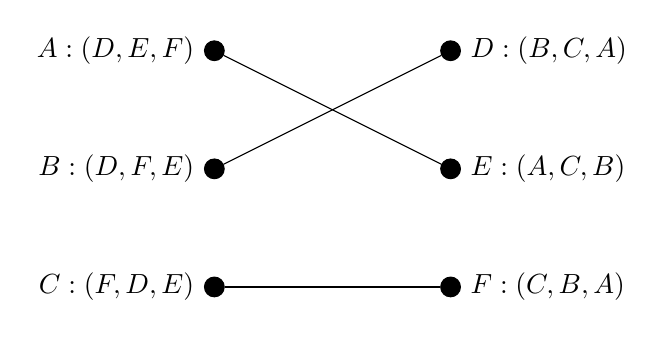
\begin{tikzpicture}[scale=0.5]

    % Suitors
    \node[draw, shape=circle, fill, inner sep=0, minimum size=0.25cm, 
    label=left: {\(A: (D, E, F)\)}] (A) at (0, 0) {};
    \node[draw, shape=circle, fill, inner sep=0, minimum size=0.25cm, 
    label=left: {\(B: (D, F, E)\)}] (B) at (0, -3) {}; 
    \node[draw, shape=circle, fill, inner sep=0, minimum size=0.25cm, 
    label=left: {\(C: (F, D, E)\)}] (C) at (0, -6) {};

    % Reviewers
    \node[draw, shape=circle, fill, inner sep=0, minimum size=0.25cm, 
    label=right: {\(D: (B, C, A)\)}] (D) at (6, 0) {};
    \node[draw, shape=circle, fill, inner sep=0, minimum size=0.25cm, 
    label=right: {\(E: (A, C, B)\)}] (E) at (6, -3) {};
    \node[draw, shape=circle, fill, inner sep=0, minimum size=0.25cm,
    label=right: {\(F: (C, B, A)\)}] (F) at (6, -6) {};

    % Lines
    \draw (A) -- (E);
    \draw (B) -- (D);
    \draw (C) -- (F);

\end{tikzpicture}
\caption{An example of a stable matching for our
    game.}\label{fig:stable_matching}

    \end{figure}
\end{example}


\subsection{The Gale-Shapley algorithm}\label{subsec:galeshapley}

The Gale-Shapley algorithm is known to find a unique stable matching for any 
matching game of size \(N\). This matching is also considered to be 
suitor-optimal. That is, each suitor is matched with the best possible reviewer
that ensures a stable matching, but is in fact the worst possible matching for 
the reviewers. \textcolor{red}{[cite or have these theorems stated/proven]} 

As was discussed at the start of Section~\ref{sec:matching}, the outline of
the method proposed in this paper is to extend Huang's method by considering the
virtual modes with some subset of the data as a matching game to be solved. It
should be noted, however, that in this method we may not have equally sized 
sets of suitors and reviewers. As a result of this, the Gale-Shapley algorithm 
becomes inapplicable as the matching produced \(M\) would not be a bijection of 
our suitors and reviewers.

\subsection{The capacitated Gale-Shapley algorithm for the hospital-resident 
	problem}\label{subsec:capacitated_galeshapley}

The situation where a large set of suitors are to be matched with a number
reviewers is not limited to abstraction. A practical example of this problem is
how to best assign a cohort of medical students to a group of hospitals. Here, 
we have all of the requisite components of a matching game:

\begin{itemize}
	\item A set of reviewers (the hospitals) and a set of suitors (the potential
        residents) 
	\item A ranking of the students/residents by the hospitals, and vice versa
\end{itemize}

The only obstacle which stops us from using the Gale-Shapley algorithm is the 
disparity in the sizes of our sets. In reality, hospitals need not always take 
at most one resident on from a cohort of medical students. So each hospital has
a capacity associated with it and we can consider our matching game to be
`capacitated'. By this we mean that each reviewer (hospital) may be matched with
any number of suitors (students) up to their capacity, making our matching
\(M:~S~\to~R\) surjective.

Research surrounding the hospital-resident assignment problem is well-documented 
\textcolor{red}{[cite]} and an extension of the Gale-Shapley algorithm was
developed to solve it, awarding the authors the 2012 Nobel Prize in Economic
Sciences. This algorithm is currently used by the National Resident Matching
Program (\url{http://www.nrmp.org}) to assign medical students to hospitals in
the United States of America.

As before, we consider a set of suitors and reviewers denoted by \(S\) and 
\(R\). These sets are no longer (necessarily) the same size. We also have our 
preference lists \(f, g\), and a set \(C = \{c_1, \ldots, c_{|R|}\}\) of 
reviewer capacities. Finally, let \(S_u \subset S\) denote the set of suitors 
that are currently unmatched. The capacitated Gale-Shapley algorithm is given 
below.

\balg%
    \caption{The hospital-resident algorithm
        (resident-optimal)}\label{alg:hospital_resident}
    \KwIn{a set of residents \(R\), a set of hospitals \(H\), a set of hospital
        capacities \(C\), two preference list functions \(f, g\)}
    \KwOut{a stable, resident-optimal mapping \(M\) between \(R\) and \(H\)}

    \For{\(h \in H\)}{%
        \(M^{-1}(h) \gets \emptyset\)
    }
    \While{There exists any unmatched \(r \in R\) with a non-empty preference
        list}{%
        Take any such resident \(r\) and their most preferred hospital \(h\)\;
        \(\textsc{MatchPair}(s, h)\)\;

        \If{\(\abs*{M^{-1}(h)} > c_h\)}{%
            Find their worst match \(r' \in M^{-1}(h)\)\;
            \(\textsc{UnmatchPair}(r', h)\)\;
        }
        \If{\(\abs*{M^{-1}(h)} = c_h\)}{%
            Find their worst match \(r' \in M^{-1}(h)\)\;
            \For{each successor \(s \in g(h)\) to \(r'\)}{%
                \(\textsc{DeletePair}(s, h)\)
            }
        }
    }
\ealg%

\balg%
    \caption{\textsc{MatchPair}}\label{alg:match}
    \KwIn{a resident \(r\), a hospital \(h\), a matching \(M\)}
    \KwOut{an updated matching \(M\)}

    \(M^{-1}(h) \gets M^{-1}(h) \cup \left\{r\right\}\)\;
\ealg%

\balg%
    \caption{\textsc{UnmatchPair}}\label{alg:unmatch}
    \KwIn{a resident \(r\), a hospital \(h\), a matching \(M\)}
    \KwOut{an updated matching \(M\)}

    \(M^{-1}(h) \gets M^{-1}(h) \setminus \left\{r\right\}\)\;
\ealg%

\balg%
    \caption{\textsc{DeletePair}}\label{alg:delete}
    \KwIn{a resident \(r\), a hospital \(h\)}
    \KwOut{updated preference lists}

    \(f(r) \gets f(r) \setminus \left\{h\right\}\)\;
    \(g(h) \gets g(h) \setminus \left\{r\right\}\)\;
\ealg%


\section{Matching games and the proposed method}\label{sec:method}

Both of the initialisation methods described in Section~\ref{subsec:inits} have
a greedy component. Cao's method essentially chooses the densest point that has
not already been chosen whilst forcing separation between the set of initial
modes. In the case of Huang's, however, the greediness only comes at the end
of the method, after the set of potential modes has been found by random
sampling.  In any practical implementation of this method, the order in which a
set of potential modes is iterated over has no guarantee of consistency. The
same is true for any arbitrary tie breaks. The result of this is that the
initial set of modes that the method returns is altered since the next initial
mode is chosen by the next locally optimal choice.

The initialisation method proposed in this work aims to extend Huang's method to
be order-invariant in the final allocation \-- thereby eliminating its greedy
component \-- and to provide a more intuitive starting point for the \(k\)-modes
algorithm. This is done by constructing and solving a matching game between the
set of potential modes and some subset of the data.

In general, matching games are defined by two sets (parties) of players (often
termed suitors and reviewers) in which each player creates a preference list of
at least some of the players in the other party. The objective then is to find a
mapping between the two sets of players such that no pair of players is
(rationally) unhappy with their matching. Such a mapping is considered stable.
Algorithms to find stable matchings to instances of matching games are often
structured to be party-oriented and aim to maximise some form of social or
party-based optimality~\cite{Fuku2006,Gale1962,Kwanashie2015}.

One of the simplest matching games models the Stable Marriage Problem (SM). In
this game the sets of players must be of equal size and rank each other strictly
(i.e.\ no ties allowed) and entirely. An algorithm was presented in the seminal
work by D.\ Gale and L.\ Shapley~\cite{Gale1962} that `solves' any instance of
SM by finding for it a unique, suitor-optimal, stable matching. This kind of
game is not considered in this work as it effectively reduces down to Huang's
method. This can be seen as follows. Note that the concept of preference between
points in an attribute space is synonymous with similarity. Thus, when
constructing the game, each potential mode gets to pick the data point it is
closest to but that has not already been picked. Then, up to an arbitrary
breaking of any ties in the preference lists, each potential mode is assigned to
its chosen data point.

A number of issues arise from this particular model other than it reducing to
Huang's method. For instance:
\begin{itemize}
    \item Ties are common when using the distance metric defined
        in~(\ref{eq:dissim}).
    \item There is no intuitively concrete way of constructing sets of players
        or their preference lists.
\end{itemize}

Allowing for ties is a simple extension to SM but the notion of stability
becomes tiered~\cite{Manlove1999}. In each case of stability, if such a matching
exists, then a polynomial-time algorithm will find one that is optimal for one
set of players. However, there is no guarantee that such a level-of-stable
matching exists and even in that case, the notion of party-optimality is
lost~\cite{Erdil2017}. Therefore this extension is not considered here where a
stable solution to the game is required, and is preferably party-optimal.

Further to allowing ties, how preference lists are constructed is a point of
interest in many applications of matching games~\cite{Iwama2008}. Often this is
a contextual problem and may be addressed in a number of ways. As in this case,
where similarity and preference are considered equivalent, a bespoke distance
metric may be used. Though not relevant to this work, if the game forms part of
a larger, long-standing or otherwise complex model, introducing flexibility in
preferences~\cite{Agarwal2017,Menzel2015} or estimating them
\emph{ad hoc}~\cite{Rastegari2016} may be helpful to obtain meaningful
matchings.

Another method used to construct preference lists is to discount the preference
lists presented by players. For instance, where acceptability of another player
is the only criterion, binary preferences (i.e.\ incomplete preference lists
with ties) can create games that are invulnerable to manipulative players'
strategies~\cite{Bogomolnaia2004}. This approach can be adapted to cater for
larger games, such as student-school allocation. In this case, each student
submits a set of acceptable schools and the schools form strict rankings of the
students. The result of this is a simpler game (in the practical sense) and a
reduction in the set of possible stable matchings~\cite{Haeringer2014}.

As this particular case has no interactive element, and must guarantee a stable
matching (ideally with optimality), none of these extensions are used in the
proposed method. Instead, so as to keep the method as simple as possible within
these constraints, the game used will model an instance of the Hospital-Resident
Assignment Problem (HR) which was presented with SM as a practical solution to
the problem that gives it its namesake~\cite{Gale1962}.

Like SM, there exists an algorithm that can provide a unique, party-optimal,
stable matching to any instance of HR.\ The resident-optimal algorithm is
presented in Algorithm~\ref{alg:hospital_resident} and is adapted from the
original to take advantage of the structure of the game~\cite{Roth1984}. The
game used to model HR, its matchings, and its notion of stability are defined in
Definitions~\ref{def:game}~\--~\ref{def:blocking}. A summary of these
definitions in the context of the proposed \(k\)-modes initialisation is given
in Table~\ref{tab:components}.

\begin{definition}\label{def:game}
    Consider two distinct sets \(R, H\) and refer to them residents and
    hospitals. Each \(h \in H\) has a capacity \(c_h \in \mathbb{N}\) associated
    with them. Each player \(r \in R\) and \(h \in H\) has associated 
    with it a strict preference list of the other set's elements such that:
    \begin{itemize}
        \item Each \(r \in R\) ranks a non-empty subset of \(H\), denoted by
            \(f(r)\).
        \item Each \(h \in H\) ranks all and only those residents that have
            ranked it, i.e.\ the preference list of \(h\), denoted \(g(h)\), is
            a permutation of the set
            \(\left\{r \in R \ | \ h \in f(r)\right\}\). If no such residents
            exist, \(h\) is removed from \(H\).
    \end{itemize}

    This construction of residents, hospitals, capacities and preference lists
    is called a \emph{game} and is denoted by \((R, H)\).
\end{definition}

\begin{definition}\label{def:matching}
    Consider a game \((R, H)\). A \emph{matching} \(M\) is any mapping between
    \(R\) and \(H\). If a pair \((r, h) \in R \times H\) are matched in \(M\)
    then this relationship is denoted \(M(r) = h\) and \(r \in M^{-1}(h)\).

    A matching is only considered \emph{valid} if all of the following hold for
    all \(r \in R, h \in H\):
    \begin{itemize}
        \item If \(r\) is matched then \(M(r) \in f(r)\).
        \item If \(h\) has at least one match then \(M^{-1}(h) \subseteq g(h)\).
        \item \(h\) is not over-subscribed, i.e.\ \(\abs*{M^{-1}(h)} \leq c_h\).
    \end{itemize}

    A valid matching is considered \emph{stable} if it does not contain any
    blocking pairs.
\end{definition}

\begin{definition}\label{def:blocking}
    Consider a game \((R, H)\). Then a pair \((r, h) \in R \times H\) is said to
    \emph{block} a matching \(M\) if all of the following hold:
    \begin{itemize}
        \item There is mutual preference, i.e.\ \(r \in g(h)\) and \(h \in
            f(r)\).
        \item Either \(r\) is unmatched or they prefer \(h\) to \(M(r)\).
        \item Either \(h\) is under-subscribed or \(h\) prefers \(r\) to at
            least one resident in \(M^{-1}(h)\).
    \end{itemize}
\end{definition}

\begin{table}[htbp]
    \resizebox{\textwidth}{!}{%
    \begin{tabular}{lcr}
        \toprule%
        Object in \(k\)-modes initialisation & {} & Object in a matching game
        \\\midrule%
        Similarity between two points \(U, V \in \mathcal{A}\),
        \(m - d\left(U, V\right)\) & {} & Respective position in preference
        lists \(f, g\)
        \\
        Potential modes, \(\widehat Z\) & {} & Residents, \(R\)
        \\
        Data points closest to \(\widehat Z\), \(\mathcal{X}' \subset
        \mathcal{X}\) & {} & Hospitals, \(H\)
        \\
        A mode \(\hat{z} \in \widehat Z\) being replaced by a point \(X \in
        \mathcal{X}'\) & {} & A pair in some matching \(M\)\\
        \bottomrule
    \end{tabular}}
    \caption{A summary of the relationships between the components of the
             initialisation for \(k\)-modes and those in a matching game
             \((R, H)\).
    }\label{tab:components}
\end{table}

%\begin{example}\label{example:matching}
    Consider the following example with \(S = \{A, B, C\}\) and \(R = \{D, E,
    F\}\). We can visualise this matching game as a bipartite graph as in
    Figure~\ref{fig:matching_bipartite}. In this representation, an edge between
    two vertices indicates that they are matched by \(M\). Beside each node is 
    the name of the node and a complete ranking of its complementary set's 
    elements. We interpret these rankings as the values of our preference list 
    functions. Here, for instance, \(A\) would most prefer to be matched with 
    \(D\), then \(E\), and finally \(F\).
    
    \begin{figure}[h]
        \centering
        \input{tex/matching_bipartite.tex}
    \end{figure}

    Suppose we have the matching shown in Figure~\ref{fig:unstable_matching} for
    our game. This matching, \(M\) is valid since it is a bijection between 
    \(S\) and \(R\) but it is not stable. For instance, we have \((B, D)\) as a
    blocking pair since \(B\) would rather be matched with \(D\) than its 
    current match \(E\), and \(D\) would prefer to be matched with \(B\) than
    its current match \(A\).

    \begin{figure}[h]
        \centering
        \input{tex/unstable_matching.tex}
    \end{figure}

    We can make this matching stable by switching these pairs as in
    Figure~\ref{fig:stable_matching}. Here we have that each suitor is matched 
    with their most preferred reviewer so as not to form a blocking pair. We 
    call such a matching \emph{suitor-optimal}.

    \begin{figure}[h]
        \centering
        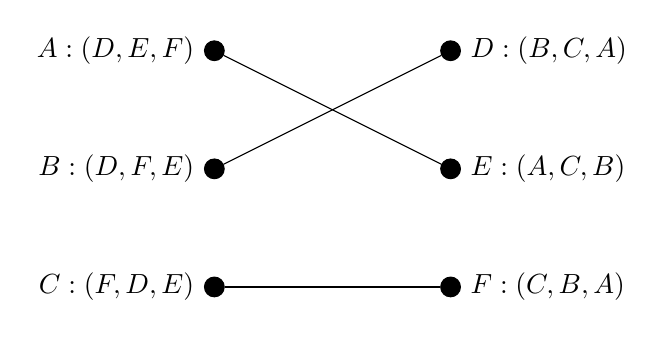
\begin{tikzpicture}[scale=0.5]

    % Suitors
    \node[draw, shape=circle, fill, inner sep=0, minimum size=0.25cm, 
    label=left: {\(A: (D, E, F)\)}] (A) at (0, 0) {};
    \node[draw, shape=circle, fill, inner sep=0, minimum size=0.25cm, 
    label=left: {\(B: (D, F, E)\)}] (B) at (0, -3) {}; 
    \node[draw, shape=circle, fill, inner sep=0, minimum size=0.25cm, 
    label=left: {\(C: (F, D, E)\)}] (C) at (0, -6) {};

    % Reviewers
    \node[draw, shape=circle, fill, inner sep=0, minimum size=0.25cm, 
    label=right: {\(D: (B, C, A)\)}] (D) at (6, 0) {};
    \node[draw, shape=circle, fill, inner sep=0, minimum size=0.25cm, 
    label=right: {\(E: (A, C, B)\)}] (E) at (6, -3) {};
    \node[draw, shape=circle, fill, inner sep=0, minimum size=0.25cm,
    label=right: {\(F: (C, B, A)\)}] (F) at (6, -6) {};

    % Lines
    \draw (A) -- (E);
    \draw (B) -- (D);
    \draw (C) -- (F);

\end{tikzpicture}
\caption{An example of a stable matching for our
    game.}\label{fig:stable_matching}

    \end{figure}
\end{example}


\balg%
    \caption{The hospital-resident algorithm
        (resident-optimal)}\label{alg:hospital_resident}
    \KwIn{a set of residents \(R\), a set of hospitals \(H\), a set of hospital
        capacities \(C\), two preference list functions \(f, g\)}
    \KwOut{a stable, resident-optimal mapping \(M\) between \(R\) and \(H\)}

    \For{\(h \in H\)}{%
        \(M^{-1}(h) \gets \emptyset\)
    }
    \While{There exists any unmatched \(r \in R\) with a non-empty preference
        list}{%
        Take any such resident \(r\) and their most preferred hospital \(h\)\;
        \(\textsc{MatchPair}(s, h)\)\;

        \If{\(\abs*{M^{-1}(h)} > c_h\)}{%
            Find their worst match \(r' \in M^{-1}(h)\)\;
            \(\textsc{UnmatchPair}(r', h)\)\;
        }
        \If{\(\abs*{M^{-1}(h)} = c_h\)}{%
            Find their worst match \(r' \in M^{-1}(h)\)\;
            \For{each successor \(s \in g(h)\) to \(r'\)}{%
                \(\textsc{DeletePair}(s, h)\)
            }
        }
    }
\ealg%

\balg%
    \caption{\textsc{MatchPair}}\label{alg:match}
    \KwIn{a resident \(r\), a hospital \(h\), a matching \(M\)}
    \KwOut{an updated matching \(M\)}

    \(M^{-1}(h) \gets M^{-1}(h) \cup \left\{r\right\}\)\;
\ealg%

\balg%
    \caption{\textsc{UnmatchPair}}\label{alg:unmatch}
    \KwIn{a resident \(r\), a hospital \(h\), a matching \(M\)}
    \KwOut{an updated matching \(M\)}

    \(M^{-1}(h) \gets M^{-1}(h) \setminus \left\{r\right\}\)\;
\ealg%

\balg%
    \caption{\textsc{DeletePair}}\label{alg:delete}
    \KwIn{a resident \(r\), a hospital \(h\)}
    \KwOut{updated preference lists}

    \(f(r) \gets f(r) \setminus \left\{h\right\}\)\;
    \(g(h) \gets g(h) \setminus \left\{r\right\}\)\;
\ealg%

\balg%
    \caption{The proposed initialisation method}\label{alg:proposed_method}
    \KwIn{a dataset \(\mathcal{X} \subset \mathcal{A}\), a number of modes to
        find \(k\)}
    \KwOut{a set of \(k\) initial modes \(\overline Z\)}

    \(\overline Z \gets \emptyset\)\;
    \(H \gets \emptyset\)\;
    \(R \gets \textsc{SamplePotentialModes}\left(\mathcal{X}\right)\)\;

    \For{\(r \in R\)}{%
        Find the set of \(k\) data points \(H_r \subset \mathcal{X}\) that 
        are the least dissimilar to \(r\)\;
        Arrange \(H_r\) into descending order of similarity with respect to
        \(r\), denoted by \(H_r^*\)\;
        \(H \gets H \cup H_r\)\;
        \(f(r) \gets H_r^*\)\;
    }

    \For{\(h \in H\)}{%
        \(c_h \gets 1\)\;
        Sort \(R\) into descending order of similarity with respect to \(h\),
        denoted by \(R^*\)\;
        \(g(h) \gets R^*\)
    }

    Solve the matching game defined by \((R, H)\) to obtain a matching \(M\)\;
    \For{\(r \in R\)}{%
        \(\overline Z \gets \overline Z \cup \left\{M(r)\right\}\)
    }
\ealg%


\section{Resident preference lists}\label{sec:preferences}

For the purposes of this piece of work and to demonstrate how preference lists
can be generated, a small number will be defined and used. While these
preference lists do not necessarily hold any mathematical justification for why
they could be appropriate or useful at all, they are the simplest methods
available. In fact, research into this area could prove to be promising as a
means of incorporating prior or expert knowledge into the clustering algorithm.

\begin{definition}\label{def:preferences}
    The three preference list methods to be used will be referred to as `Best',
    `Worst' and `Random' from this point, most notably in
    Section~\ref{sec:results}. Their definitions are somewhat self-explanatory
    but are given below.

    Let \((S, R, C)\) be a capacitated matching game where \(R = \tilde{\mu}\)
    and \(S = \left\{S_r : r \in R\right\}\) as in the proposed method. Then the
    reviewer-suitor preference function \(g\) is well-defined by the proposed
    method. Consider some \(s \in S\). Then their preference function \(f(s)\)
    could be defined in the following way:
    \begin{itemize}
        \item \textbf{Best:} Rank the elements of \(R\) in \emph{ascending}
            order of dissimilarity with respect to \(s\) and set this to be
            \(f(s)\).
        \item \textbf{Worst:} Rank the elements of \(R\) in \emph{descending}
            order of dissimilarity with respect to \(s\) and set this to be
            \(f(s)\).
        \item \textbf{Random:} Take a random permutation of the elements of
            \(R\) and set this to be \(f(s)\).
    \end{itemize}
\end{definition}

\begin{remark}
    It should be noted that `Best' could be considered the greediest approach to
    take since it involves choosing the most preferred option for each of the
    slots available in the list. `Random' should also be expected to perform
    badly on average since it creates an element of stupidity in a method that
    is intended to be an intelligent cluster selection. `Worst' is included to
    observe the effects of deliberately choosing a preference list that goes
    against common sense approaches.

    Note also that each of these preference list operators requires a suitor to
    rank all of the reviewers. A slight modification to some (such as the
    inclusion of a threshold on dissimilarity) could drastically improve their
    performance. Also, it is possible to generate a preference list such that
    the proposed method produces an initial clustering identical to that found
    by Huang's method, though that is not discussed here as it has been
    considered trivial.
\end{remark}

\section{Experimental results}\label{sec:results}

To give comparative results on the quality of the initialisation processes 
defined in
Sections~\ref{sec:init},~\ref{sec:proposed-method}~\&~\ref{sec:preferences},
four well-known, categorical, labelled datasets \- soybean, mushroom, breast
cancer, and zoo animal \- will be clustered by the \(k\)-modes algorithm with
each of the initialisation processes using their respective number of classes as
the number of clusters. These datasets have been chosen to fall in line with the
established literature, and for their relative sizes and complexities.

Typically, the quality of a clustering algorithm is measured by its performance
at classifying datasets~\cite{Huang1998}\cite{Cao2009}~\cite{Olaode2014}. In
this work, however, we will not follow this approach since our motivation is to
compare the quality of the clustering produced when using these initialisation
methods. So, for the purposes of measuring the performance of our various
initialisation methods as parts of a clustering algorithm, we will make use of
internal metrics that are independent of any external information such as a
class labelling. This family of metrics are built up from two characteristics of
the clusters found: cohesion and separation. Cluster cohesion is effectively the
summed, within-cluster variation or dissimilarity of its points, whereas a
cluster's separation is a sum of the distances between all points in the cluster
and every other point not in the cluster. In this analysis, we will make use of
two internal measures for cluster validity: our cost function from
Definition~\ref{def:cost} and the average silhouette coefficient, or silhouette
score, of our clustering, defined below. 

\begin{definition}\label{def:silhouette}
    Let \textbf{X} be a dataset and consider a clustering of \textbf{X} into
    \(k\) parts, denoted by \(C = \left\{C_1, \ldots, C_k\right\}\). For each
    \(X^{(i)} \in \textbf{X}\), we define the following two quantities:
    \begin{itemize}
        \item Let \(a\left(X^{(i)}\right)\) denote the average dissimilarity
            between \(X^{(i)}\) and every other point in its cluster. Without
            loss of generality, let \(X^{(i)} \in C_l\). Then:
            \[
                a\left(X^{(i)}\right) := \frac{1}{|C_l|} D\left(C_l,
                X^{(i)}\right)
            \]
        \item Let \(b\left(X^{(i)}\right)\) denote the lowest average 
            dissimilarity between \(X^{(i)}\) and all other points in each
            cluster other than \(C_l\). That is:
            \[
                b\left(X^{(i)}\right) := \min_{l' \neq l} \left\{
                \frac{1}{|C_{l'}|} D\left(C_{l'}, X^{(i)}\right) \right\}
            \]\\
    \end{itemize}

    With these quantities we define, for each point in our datset, their
    \emph{silhouette coefficient}, denoted by \(s(X^{(i)})\):
    \[
        s(X^{(i)}) := \frac{b\left(X^{(i)}\right) -
        a\left(X^{(i)}\right)}{\max\left\{a\left(X^{(i)}\right),
        b\left(X^{(i)}\right)\right\}}
    \]

    The \emph{silhouette score} of a clustering \(C\) is simply the average of
all the silhouette coefficients. Silhouette scores take value in the range
\([-1, 1]\). Negative scores generally suggest that elements in the data have
been mis-clustered since there exists a closer cluster centre than its own.
Values around 0 indicate overlapping clusters, whereas silhouette scores close
to 1 suggest well-separated and effective clusters.
\end{definition}


\subsection{The datasets}\label{subsec:datasets}

As stated above, the datasets being used for this work are well-known and openly
available. Below is a summary of their properties and access links for each.

\subsubsection*{Soybean}

The soybean dataset describes 35 characteristics of 307 soybean instances to
classify which disease is present. The attributes are encoded numerically as
integers but will be considered as strings for this analysis.
The diseases form .8 classes, though the first 15 are the only ones used since
they contain a considerable number of instances each~\cite{Soybean}. 
Available~at:~\url{https://archive.ics.uci.edu/ml/datasets/Soybean+(Large)}.

\subsubsection*{Mushroom}

The mushroom dataset was constructed to classify 8124 mushroom instances forming
23 species found in North America into two classes: edible and poisonous. The
attributes describe the physical characteristics and habitat of the mushrooms,
and are encoded as strings~\cite{Mushroom}. Available~at:~\url{https://archive.
ics.uci.edu/ml/datasets/mushroom}.

\subsubsection*{Breast cancer}

Wisconsin University constructed the breast cancer dataset using a decision tree
with linear programming as a diagnostic tool. The features were created using
digital images of a fine needle aspirate of a breast mass to describe the
structure of cell nuclei. There are 5.8 instances and 32 attributes in total.
Available~upon~request~to~members~of~the~academic~community~at:~\url{https://
archive.ics.uci.edu/ml/datasets/Breast+Cancer+Wisconsin+(Diagnostic)}.

\subsubsection*{Zoo animal}

The zoo animal dataset is an entirely artificial dataset used to classify 101
animals into 7 classes, those being mammal, reptile, amphibian, bird, fish,
insect, and crustacean. The 17 attributes include the name of the animal and a
series of Boolean variables describing characteristics and the habitat of the
animals. Available~at:~\url{http://archive.ics.uci.edu/ml/datasets/zoo}.

\subsection{Results}\label{subsec:results}

In this section, two sets of results will be considered. The first are the more
classically seen tables of metrics defined above, and the latter are a
collection of plots showing the descent in the cost function of the \(k\)-modes
algorithm over time. In either case, results are generated using the Python
library \href{https://github.com/nicodv/kmodes}{\texttt{kmodes}} to which the
proposed method has been added as another initialisation method. The number of
clusters to be determined, \(k\), is chosen as the number of classes associated
with each dataset. Note that this value may not be optimal (as suggested by the
relatively low silhouette scores in most cases), and that the class variable is
not considered in the running of the algorithm.

\subsubsection{Metric results}

Each of the tables of results given below were obtained by running the
\(k\)-modes algorithm 25 times with each initialisation method on the dataset in
question. For each of these 25 runs, the simulation is seeded to make the
results reproducible.

At each run of the experiment the number of epochs to termination, the initial
and final costs, and the average silhouette score were recorded for the
clustering found. These metrics are summarised below in
Tables~\ref{tab:soybean_results}~\--~\ref{tab:zoo_animal_results} by their mean
and median values, and their standard deviation over the 25 runs.

\singlespacing%
\begin{table}[H]
    \centering
    \resizebox{.9\textwidth}{!}{%
        \begin{tabular}{llrrrr}
\toprule
Initialisation & {} &  No. of iterations &  Initial cost &  Final cost &  Silhouette score \\
\midrule
Cao & mean &             2.0000 &     1574.0000 &   1314.0000 &            0.2349 \\
    & median &             2.0000 &     1574.0000 &   1314.0000 &            0.2349 \\
    & std &             0.0000 &        0.0000 &      0.0000 &            0.0000\\
\midrule
Huang & mean &             3.7600 &     1795.4400 &   1455.3200 &            0.1212 \\
    & median &             4.0000 &     1830.0000 &   1428.0000 &            0.1234 \\
    & std &             1.0520 &      131.9621 &     72.7637 &            0.0357 \\
\midrule
Matching Best & mean &             3.6800 &     1773.2400 &   1449.6400 &            0.1205 \\
    & median &             3.0000 &     1781.0000 &   1443.0000 &            0.1193 \\
    & std &             1.1075 &      118.8992 &     63.0971 &            0.0247 \\
\midrule
Matching Random & mean &             3.8800 &     1774.3600 &   1438.8000 &            0.1237 \\
    & median &             4.0000 &     1780.0000 &   1431.0000 &            0.1291 \\
    & std &             1.0924 &      121.9911 &     54.0301 &            0.0234 \\
\midrule
Matching Worst & mean &             4.0400 &     1774.9600 &   1431.8400 &            0.1290 \\
    & median &             4.0000 &     1777.0000 &   1430.0000 &            0.1291 \\
    & std &             1.0985 &      123.0411 &     53.9859 &            0.0248 \\
\midrule
Random & mean &             3.6800 &     1638.8000 &   1351.2400 &            0.1608 \\
    & median &             3.0000 &     1626.0000 &   1345.0000 &            0.1620 \\
    & std &             1.1804 &       98.2480 &     36.3126 &            0.0312 \\
\bottomrule
\end{tabular}

    }
    \captionof{table}{Summative metric results for the soybean dataset with
    \(k=15\).}\label{tab:soybean_results}\vspace{20pt}

    \resizebox{.9\textwidth}{!}{%
        \begin{tabular}{llrrrr}
\toprule
Initialisation & {} &  No. of iterations &  Initial cost &  Final cost &  Silhouette score \\
\midrule
Cao & mean &             2.0000 &    63242.0000 &  62644.0000 &            0.2517 \\
    & median &             2.0000 &    63242.0000 &  62644.0000 &            0.2517 \\
    & std &             0.0000 &        0.0000 &      0.0000 &            0.0000 \\
\midrule
Huang & mean &             2.8400 &    75107.8400 &  63231.8400 &            0.2274 \\
    & median &             3.0000 &    76026.0000 &  63002.0000 &            0.2179 \\
    & std &             0.9866 &     5864.1758 &   1059.4049 &            0.0332 \\
\midrule
Matching Best & mean &             2.8400 &    74822.2800 &  63319.5600 &            0.2209 \\
    & median &             3.0000 &    75192.0000 &  63015.0000 &            0.2179 \\
    & std &             1.0279 &     4914.2731 &   1186.2087 &            0.0345 \\
\midrule
Matching Random & mean &             2.8400 &    74822.2800 &  63319.5600 &            0.2209 \\
    & median &             3.0000 &    75192.0000 &  63015.0000 &            0.2179 \\
    & std &             1.0279 &     4914.2731 &   1186.2087 &            0.0345 \\
\midrule
Matching Worst & mean &             2.8400 &    74822.2800 &  63319.5600 &            0.2209 \\
    & median &             3.0000 &    75192.0000 &  63015.0000 &            0.2179 \\
    & std &             1.0279 &     4914.2731 &   1186.2087 &            0.0345 \\
\midrule
Random & mean &             2.6400 &    78345.8400 &  63824.8000 &            0.2243 \\
    & median &             2.0000 &    78603.0000 &  63155.0000 &            0.2281 \\
    & std &             0.8103 &     6146.4742 &   1684.9847 &            0.0391 \\
\bottomrule
\end{tabular}

    }
    \captionof{table}{Summative metric results for the mushroom dataset with
    \(k=2\).}\label{tab:mushroom_results}
\end{table}

\begin{table}[H]
    \centering
    \resizebox{.9\textwidth}{!}{%
        \begin{tabular}{llrrrr}
\toprule
Initialisation & {} &  No. of iterations &  Initial cost &  Final cost &  Silhouette score \\
\midrule
Cao & mean &             3.0000 &     3546.0000 &   3250.0000 &            0.3453 \\
    & median &             3.0000 &     3546.0000 &   3250.0000 &            0.3453 \\
    & std &             0.0000 &        0.0000 &      0.0000 &            0.0000 \\
\midrule
Huang & mean &             2.0400 &     3809.3200 &   3428.3200 &            0.1655 \\
    & median &             2.0000 &     3846.0000 &   3492.0000 &            0.0933 \\
    & std &             0.4546 &      206.2981 &    151.9832 &            0.1595 \\
\midrule
Matching Best & mean &             2.0400 &     3804.7200 &   3386.4000 &            0.1943 \\
    & median &             2.0000 &     3803.0000 &   3257.0000 &            0.3439 \\
    & std &             0.4546 &      177.0794 &    146.2635 &            0.1681 \\
\midrule
Matching Random & mean &             2.0400 &     3804.7200 &   3386.4400 &            0.1940 \\
    & median &             2.0000 &     3803.0000 &   3257.0000 &            0.3439 \\
    & std &             0.4546 &      177.0794 &    146.2247 &            0.1677 \\
\midrule
Matching Worst & mean &             2.0400 &     3804.7200 &   3386.4400 &            0.1940 \\
    & median &             2.0000 &     3803.0000 &   3257.0000 &            0.3439 \\
    & std &             0.4546 &      177.0794 &    146.2247 &            0.1677 \\
Random & mean &             2.0400 &     4150.8000 &   3349.9200 &            0.2338 \\
    & median &             2.0000 &     3682.0000 &   3250.0000 &            0.3453 \\
    & std &             0.3512 &      828.8702 &    136.8819 &            0.1631 \\
\bottomrule
\end{tabular}

    }
    \captionof{table}{Summative metric results for the breast cancer dataset
    with \(k=2\).}\label{tab:breast_cancer_results}\vspace{20pt}

    \resizebox{.9\textwidth}{!}{%
        \begin{tabular}{llrrrr}
\toprule
Initialisation & {} &  No. of iterations &  Initial cost &  Final cost &  Silhouette score \\
\midrule
Cao & mean &             2.0000 &      377.0000 &    232.0000 &            0.3860 \\
    & median &             2.0000 &      377.0000 &    232.0000 &            0.3860 \\
    & std &             0.0000 &        0.0000 &      0.0000 &            0.0000 \\
\midrule
Huang & mean &             2.4800 &      360.2800 &    250.3200 &            0.3047 \\
    & median &             2.0000 &      358.0000 &    244.0000 &            0.3271 \\
    & std &             0.6532 &       41.1213 &     15.2226 &            0.1038 \\
\midrule
Matching Best & mean &             2.3600 &      359.6800 &    251.8400 &            0.3045 \\
    & median &             2.0000 &      352.0000 &    252.0000 &            0.3184 \\
    & std &             0.4899 &       42.6602 &     12.5322 &            0.0926 \\
\midrule
Matching Random & mean &             2.4000 &      360.5200 &    252.6000 &            0.3083 \\
    & median &             2.0000 &      352.0000 &    253.0000 &            0.3300 \\
    & std &             0.5000 &       42.5853 &     12.1587 &            0.0938 \\
\midrule
Matching Worst & mean &             2.4800 &      367.0000 &    249.8800 &            0.3047 \\
    & median &             2.0000 &      356.0000 &    252.0000 &            0.3138 \\
    & std &             0.6532 &       42.7444 &      9.8375 &            0.0729 \\
\midrule
Random & mean &             2.4000 &      340.0800 &    265.2000 &            0.2658 \\
    & median &             2.0000 &      335.0000 &    253.0000 &            0.3122 \\
    & std &             0.7638 &       58.5227 &     27.1953 &            0.1204 \\
\bottomrule
\end{tabular}

    }
    \captionof{table}{Summative metric results for the zoo animal dataset with
    \(k=7\).}\label{tab:zoo_animal_results}
\end{table}
\doublespacing%

\subsubsection{Epoch costs}

The epoch-cost plots in this section were created by setting an initial seed for
each initialisation method and then running the \(k\)-modes algorithm 25 times.
Of these runs, the best set of costs is then chosen by their final cost and
plotted.

Note that in each figure, dotted lines indicate the established initialisation
methods whilst solid lines are used for the proposed method.

\begin{figure}[h!]
    \centering
    \includegraphics[width=.8\textwidth]{./img/epoch_plot_soybean.pdf}
\end{figure}

\begin{figure}[h!]
    \centering
    \includegraphics[width=.8\textwidth]{./img/epoch_plot_mushroom.pdf}
\end{figure}

\begin{figure}[h!]
    \centering
    \includegraphics[width=.8\textwidth]{./img/epoch_plot_breast_cancer.pdf}
\end{figure}

\begin{figure}[h!]
    \centering
    \includegraphics[width=.8\textwidth]{./img/epoch_plot_zoo_animal.pdf}
\end{figure}


\clearpage%
\bibliography{references}
\end{document}
